%%%%%%%%%%%%%%%%%%%%%%%%%%%%%%%%%%%%%%%%%%%%%%%%%%%%%%%%%%%%%%%%%%%%%%%%%%
%%LaTeX template for papers && theses									%%
%%Done by the incredible ||Z01db3rg||									%%
%%Under the do what ever you want license								%%
%%%%%%%%%%%%%%%%%%%%%%%%%%%%%%%%%%%%%%%%%%%%%%%%%%%%%%%%%%%%%%%%%%%%%%%%%% 

%start preamble
\documentclass[paper=a4,fontsize=11pt]{scrartcl}%kind of doc, font size, paper size
\usepackage[ngerman]{babel}%for special german letters etc			
%\usepackage{t1enc} obsolete, but some day we go back in time and could use this again
\usepackage[T1]{fontenc}%same as t1enc but better						
\usepackage[utf8]{inputenc}%utf-8 encoding, other systems could use others encoding
%\usepackage[latin9]{inputenc}			
\usepackage{amsmath}%get math done
\usepackage{amsthm}%get theorems and proofs done
\usepackage{graphicx}%get pictures & graphics done
\graphicspath{{pictures/}}%folder to stash all kind of pictures etc
\usepackage{amssymb}%symbolics for math
\usepackage{amsfonts}%extra fonts
\usepackage []{natbib}%citation style
\usepackage{caption}%captions under everything
\usepackage{listings}
\usepackage[titletoc]{appendix}
\numberwithin{equation}{section} 
\usepackage[printonlyused,withpage]{acronym}%how to handle acronyms
\usepackage{float}%for garphics and how to let them floating around in the doc
\usepackage{cclicenses}%license!
\usepackage{xcolor}%nicer colors, here used for links
\usepackage{wrapfig}%making graphics floated by text and not done by minipage
\usepackage{dsfont}
\usepackage{stmaryrd}
\usepackage{geometry}
\usepackage{hyperref}
\usepackage{fancyhdr}
\usepackage{menukeys}

%settings colors for links
\hypersetup{
    colorlinks,
    linkcolor={blue!50!black},
    citecolor={blue},
    urlcolor={blue!80!black}
}

\definecolor{pblue}{rgb}{0.13,0.13,1}
\definecolor{pgreen}{rgb}{0,0.5,0}
\definecolor{pred}{rgb}{0.9,0,0}
\definecolor{pgrey}{rgb}{0.46,0.45,0.48}

\pagestyle{fancy}
\lhead{Benjamin Tröster\\Netzwerke Übung (WiSe2018/19)}
\rhead{FB 4 -- Angewandte Informatik\\ HTW-Berlin}
\lfoot{Übungsblatt 03 -- Routing}
\cfoot{}
\fancyfoot[R]{\thepage}
\renewcommand{\headrulewidth}{0.4pt}
\renewcommand{\footrulewidth}{0.4pt}

\lstdefinestyle{Bash}{
  language=bash,
  showstringspaces=false,
  basicstyle=\small\sffamily,
  numbers=left,
  numberstyle=\tiny,
  numbersep=5pt,
  frame=trlb,
  columns=fullflexible,
  backgroundcolor=\color{gray!20},
  linewidth=0.9\linewidth,
  %xleftmargin=0.5\linewidth
  upquote=true,
  columns=fullflexible,
  literate={*}{{\char42}}1
         {-}{{\char45}}1
}

\newlength\labelwd
\settowidth\labelwd{\bfseries viii.)}
\usepackage{tasks}
\settasks{counter-format =tsk[a].), label-format=\bfseries, label-offset=3em, label-align=right, label-width
=\labelwd, before-skip =\smallskipamount, after-item-skip=0pt}
\usepackage[inline]{enumitem}
\setlist[enumerate]{% (
labelindent = 0pt, leftmargin=*, itemsep=12pt, label={\textbf{\arabic*.)}}}

\pdfpkresolution=2400%higher resolution

%%here begins the actual document%%
\newcommand{\horrule}[1]{\rule{\linewidth}{#1}} % Create horizontal rule command with 1 argument of height

\DeclareMathOperator{\id}{id}

\begin{document}
\begin{center}
\Large{\textbf{Übungsblatt 03 -- Routing}}\\
\end{center}
Nachdem Sie in der letzten Übung einige Grundlagen im Bereich Linux und Netzwerktechnik kennengelernt haben, soll im Folgenden darauf aufbauend Ihr Wissen erweitert werden. Mit diesem Hausaufgabenblatt sollen die Grundlagen für die Umsetzung eines einfachen gerouteten Netzwerks gelegt werden.\\
\begin{center}
\Large{\textbf{Aufgabe A -- Routing Grundlagen}}
\end{center}
\vskip0.25in
Nachdem Sie im letzten Übungsblatt Ihr Netzwerk durch einen Switch verbunden haben und hierdurch Ihre Kommunikation aufgebauten, \glqq wandern\grqq\ Sie im kommenden Übungsblatt im OSI-Modell eine Schicht weiter nach oben. Es soll folglich ein Netzwerk geplant sowie umgesetzt werden, das auf Routing setzt. Der Router ist fortan zentrale Anlaufstelle für die Kommunikation. Diese Umsetzung hat den Vorteil, dass der Router Pakete über Netzgrenzen hinweg vermitteln kann. Ihr kleines, abgeschottetes Netzwerk kann über die bisherigen Grenzen hinweg kommunizieren.
\begin{itemize}
	\item[1.)] Lesen Sie folgenden Artikel: \url{https://en.wikipedia.org/wiki/Routing}
	\item[2.)] Was sind die Aufgaben eines Routers. Wie erfolgt, im Groben, die Umsetzung des Routings?
	\begin{itemize}
		\item Aufgaben: Zwischenknoten im Netzwerk, weiterleiten von Paketen -- mithilfe von IP-Adressen
		\item Umsetzung: Router -- Layer 3 Gerät, arbeitet mit IP-Adressen \& Routing-Protokollen
		\item Der Router kennt das eigene Netzwerk und erkennt anhand der IP-Adresse, ob das Ziel innerhalb des eigenen Netzes liegt oder nicht
		\item Wenn keine direkte Kommunikation möglich ist, muss ein Weg in das Zielnetzwerk gefunden werden
		\item Routing-Protokolle sorgen dafür, dass eine Route vom Sender zum Empfänger gefunden wird (später mehr dazu!)
		\item Zwischenknoten, die die Pakete \glqq nur\grqq\ weiterleiten reichen Pakete nicht in höhere Schichten des OSI-Modells
		\item Im Zielnetzwerk (Router des Ziels) bestimmt Zielrechner (Endknoten) und übermittelt Pakete
	\end{itemize}
	\item[3.)] Nennen Sie einige Routing-Protokolle. Welches Protokoll ist am bekanntest für das Routing?
	\begin{itemize}
		\item IPv4
		\item IPv6
		\item BGP
		\item RIP
	\end{itemize}
	\item[4.)] Machen Sie sich klar, wie Router und Routing-Protokoll (in unserem Fall das IP-Protokoll) zusammenhängen!
	\begin{itemize}
		\item Router implementieren Routing-Protokolle, d.h. spezielle Routing-Protokolle benötigen u.U. spezielle Hard- \& Software 
	\end{itemize}
	\item[5.)] Auf welche Ebene im OSI-Modell würden Sie einen Router einordnen?
	\begin{itemize}
		\item Vermittlungsschicht (Network Layer)
	\end{itemize}
	\item[6.)] Wie haben sich bis jetzt Ihre Raspberry Pis gefunden? Woher \glqq wussten\grqq\ sie, an welches Gerät die Frames zu schicken waren? Wie spielt hier Ihre eigene IP-Adresse, Ihre Subnetzmaske mit hinein?
	\begin{itemize}
		\item Netzwerk mit Switch: Switch hält Tabelle vor, in der MAC-Adressen \& Port den jeweiligen Geräten zugeordnet wurde
		\item Adressierung aufgrund der MAC-Adressen und erfragen der IP \& MAC-Adressen
		\item IP-Adresse \& Subnetzmaske mussten vergeben werden, um das Netzwerk abzugrenzen
		\item Die Adressauflösung erfolgt mithilfe des Address Resolution Protocols (ARP), welches die Layer 2 \& 3 \glqq verbindet/ vermischt\grqq
	\end{itemize}
\end{itemize}
\begin{center}
\Large{\textbf{Aufgabe B -- Planung des Routing zwischen Netzen}}
\end{center}
\vskip0.25in
Im vorigen Aufgabenblatt haben Sie zu den IP-Adressen auch eine Netzwerkmaske konfiguriert. Diese Netzwerkmaske legt fest, welche Rechner im gleichen (Sub-)Netz liegen und somit direkt angesprochen werden können. Daraus folgt aber auch, dass bestimmte Rechner außerhalb Ihres Netzes nicht direkt angesprochen werden können. Diese können via Router/Gateway erreicht werden.\\
Wir wollen in einem ersten Schritt selber einen Router betreiben, um über unsere kleinen Netze hinweg zu kommunizieren. Dazu erweitern Sie Ihr Wissen aus dem vorigen Übungsblatt, sodass Ihr Netzwerk im Labor \glqq wachsen\grqq\ kann.
\begin{enumerate}
	\item Früher wurden Klassen von Adressen genutzt, heute wird dies nicht mehr getan. Zum Einsatz kommt die \emph{Classles Inter Domain Routing (CIDR)}. Worin unterscheiden sich \emph{CIDR} und klassenbasierte Adressen? Recherchieren Sie, warum sich dies änderte!
	\begin{itemize}
		\item Ursache: klassenbasierte Notation verschwendet häufig zu viele Adressen \footnote{IPv4 leidet seit Jahrzehnten unter einem zu kleinen Adressraum, ein Feature das mit IPv6 nicht auftreten sollte, da der Adressraum größer als die Anzahl der Atome im Universum ist.}
		\item Unterschied: klassenbasiert kennt nur feste Größen und feste Adressen, Bit-Präfix ist hier entscheidend!:
		\begin{itemize}
			\item[A] Bit-Präfix: 0, Länge 1\\
			0.0.0.0 -- 127.255.255.255, $2^7 = 128$ Netze \& $2^{24} - 2 = 16777214$ Hosts/Netz
			\item[B] Bit-Präfix: 10, Länge 2\\
			128.0.0.0 -- 191.255.255.255, $2^{14} = 16384$ Netze \& $2^{16} - 2 = 65534$Hosts/Netz 
			\item[C] Bit-Präfix: 110, Länge 3\\
			192.0.0.0 -- 223.255.255.255, $2^{21} = 2097152$ Netze \& $2^8 - 2 = 254$ Hosts/Netz
			\item[D] Bit-Präfix: 1110, Länge 4\\
			224.0.0.0 -- 239.255.255.255, $2^{28}$ = 268435456 Adressen -- MULTICAST
			\item[E] Bit-Präfix: 1111, Länge 4\\
			240.0.0.0	255.255.255.255, $2^{28} = 268435456$ Adressen -- Reserviert für \glqq zukünftiges\grqq \footnote{Der Autor kann sich einen hämischen Kommentar nicht unterdrücken: \glqq zukünftiges\grqq und IPv4, was unter Netzwerken oftmals schon als Legacy gilt. }
		\end{itemize}
		\item \emph{CIDR} ermöglicht eine feingranularere Planung \& Umsetzung von Netzwerken, d.h. weniger Verschnitt an IP-Adressen
		\item Der oben erwähnte Adressmangel wird dadurch nicht behoben, sondern nur abgemildert
	\end{itemize}
	\item Wie in der letzten Übung arbeiten Sie in Gruppen von je vier Studierenden.\\
	Um zwischen den beiden lokalen Netzwerken kommunizieren zu können benötigen Sie einen Router. Einer der Raspberry Pis soll diese Aufgabe übernehmen. Die Rechner müssen so konfiguriert werden, dass sie wissen wohin die Pakete geschickt werden -- das heißt Pakete die nicht in das eigene lokale Netzwerk gehören werden über den Router weitergereicht.
	\begin{figure}[H]
	\centering
	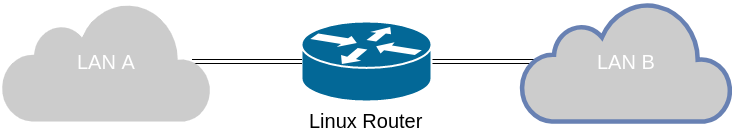
\includegraphics[scale=0.35]{lan}
	\end{figure}
	\begin{tasks}
		\task~ Unterteilen Sie Ihre Gruppe, sodass sich im Idealfall zwei Raspberry Pis in einen lokalen Netzwerk A und zwei Raspberry Pis im lokalen Netzwerk B befinden.
		\begin{table}[H]
\caption{Beispiel für ein Adressschema}
\label{adress_scheme}
\centering
\begin{tabular}{|c|c|}\hline
 & \textbf{IP-Range} \\ \hline
 Labornetz & 10.0.0.0/8 \\ \hline
 $LAN_A$ & 10.0.1.0/29 \\ \hline
 $LAN_B$ & 10.0.2.0/30 \\ \hline
 Uplink & 10.10.10.254 \\ \hline
 DNS & 10.10.10.254 \\ \hline
\end{tabular}
\end{table}
		\task~ Skizzieren Sie Ihre lokalen Netzwerke, sowie das gesamte Netzwerk.
		\task~ Vergeben Sie entsprechend IP-Adressen und kleinst mögliche Subnetzmasken auf der Skizze. Wählen Sie ein ähnliches Adressschema, wie in der letzten Laborübung.
		\task~ Planen Sie ebenso den Router mit entsprechenden IP-Adressen auf der Skizze ein. Achten Sie darauf, dass der Router als Verbindungsstück (Intermediate-Node/ Zwischenknoten) zwischen Ihren beiden Netzen fungiert und dementsprechend beide Netzwerke kennen muss. Das heißt, der Router muss zwei IP-Adressen haben, jeweils eine pro Netzwerk.
	\end{tasks}
	\begin{figure}[H]
			\centering
			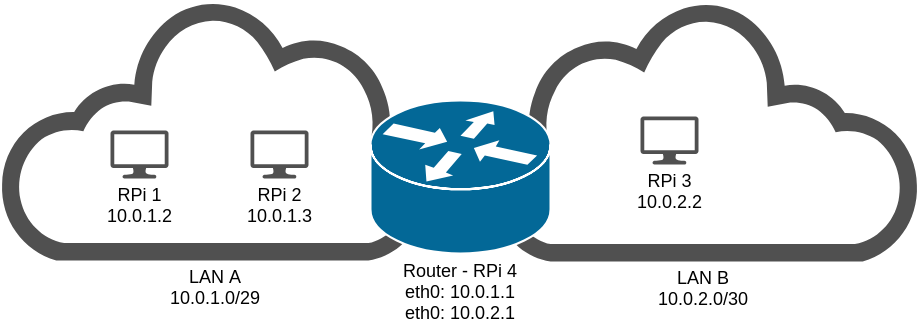
\includegraphics[scale=0.4]{example_lan}
			\caption{Skizze des Netzwerkes bestehend aus einen lokalen Netzwerk A und B, sowie einem Router der zu beiden Netzwerken gehört.}
		\end{figure}
\end{enumerate}
\begin{center}
\Large{\textbf{Aufgabe C -- Tools \& OS}}
\begin{enumerate}
	\item Seit der letzten Übung kennen Sie schon einige grundlegende Befehle, um das Netzwerkinterface eines unixoiden Betriebssystems zu konfigurieren. Dieses Wissen soll nun erweitert werden. Hierfür schauen wir in die bekannten Werkzeugkästen \emph{iproute2} und \emph{net-tools}.
	\begin{tasks}(1)
	\task~ Recherchieren Sie, welches Tool des \emph{iproute2} genutzt werden kann um Routen zu setzen. Notieren Sie sich die Syntax und was die Parameter bewerkstelligen. \footnote{Die Syntax kann anhand der Adressen der letzten Laborübung verdeutlicht werden.}
	\begin{itemize}
		\item \emph{ip route destination\_network/[subnet\_mask] \\via IP\_address\_of\_next\_hop\_neighbor dev interface\_to\_exit}
		\begin{itemize}
			\item Modifier: add -- fügt Routen in Routingtabelle hinzu, del -- löscht Eintrag, show zeigt aktuelle Tabelle an
			\item Destination: Zielnetzwerk -- welches Netzwerk soll erreichbar sein
			\item Subnetzmaske des Zielnetzes
			\item via -- über welches Gateway
			\item IP-Adresse des Gateways, muss erreichbar sein
			\item dev -- Device, über welche Schnittstelle sollen die Pakete verschickt werden
			\item Interface: bspw.: eth0 oder igb1 etc.
		\end{itemize}		 
		\item Beispiel: Von LAN A -- 10.0.1.0/29 nach LAN B -- 10.0.2.0/30\\ \emph{ip route add 10.0.2.0/30 via 10.0.1.1 dev eth0}\\
		Route von LAN A (10.0.1.0/29) in das Zielnetzwerk LAN B (10.0.2.0/30) über den Router 10.0.1.1 und über \glqq mein\grqq\ Netzwerkadapter eth0
	\end{itemize}
	\task~ Analog dazu: Wie werden Routen mithilfe der \emph{net-tools} konfiguriert?
	\begin{itemize}
		\item \emph{route add -net|host destination\_network | destinationhost \\
		netmask NETMASK gw IP\_of\_gateway}
		\item Beispiel: Von LAN A -- 10.0.1.0/29 nach LAN B -- 10.0.2.0/30\\
		\emph{route add -net 10.0.2.0 netmask 255.255.255.248 gw 10.0.1.1}
	\end{itemize}
	\task~ Recherchieren Sie beispielhaft wie eine persistente Lösung aussähe. Kommentieren Sie Ihr Beispiel anschließend, sodass Sie wissen was die einzelnen Zeilen bedeuten.\\
	\# Makiert Anfang des Kommentars -- wird von OS ignoriert
	\end{tasks}
	\begin{lstlisting}[style=Bash, language=Bash, label={netcat_server}]
auto eth0 #automatisches hochfahren von eth0
    iface eth0 inet static # interface eth0 statisch ipv4
        address 10.0.2.2 # ipv4 adresse auf eth0
        netmask 255.255.255.248 # netzwerkmaske
        gateway 10.0.2.1 # gateway -> router
		\end{lstlisting}
	\item Gateways \& Router -- Gateways sind im allgemeinen nicht das Gleiche wie Router. Auch unter den Gateways gibt es Unterscheidungen.
	\begin{tasks}(1)
	\task~ Recherchieren Sie worin sich Router und Gateways unterscheiden.
	\begin{itemize}
		\item Beide Geräte regeln die Netzwerkverkehr zwischen mehreren LANs
		\item Router regeln den Traffic zwischen gleichen Netzwerken
		\item Gateways regeln Traffic auch in heterogenen Netzwerken, d.h. Netzwerke die unterschiedliche Technologien verwenden
	\end{itemize}
	\task~ Beim aufsetzen des Netzwerkes kann unterschieden werden zwischen \emph{Gateways} und \emph{Default Gateways}. Recherchieren Sie diese Unterscheidung. Erläutern Sie die Ursache des Unterschieds.
	\begin{itemize}
		\item Gateways sind \glqq Übergangsstellen\grqq\ zwischen Netzwerken
		\item Leiten Daten weiter -- Gateways können dabei in bestimmte Netzwerke routen
		\item Default-Gateways sind die Standardgateways, welche immer dann angesprochen werden, wenn es keine andere Route für Pakete gibt
		\item D.h. sobald kein anderes Gateway weiß, wie/wohin ein Paket geroutet werden soll, dann muss sich das Default-Gateway darum kümmern
	\end{itemize}
	\end{tasks}
	\item Im vorigen Übungsblatt arbeitete Ihr Netzwerk mithilfe eines Switches. Alle Knoten des Netzwerkes waren innerhalb eines Segments (LAN). Daher konnte Sie nur innerhalb Ihres Netzwerkes kommunizieren, darüber hinaus aber nicht. Mithilfe eines Routers erweitern Sie die Reichweite Ihres Netzwerkes. Jedoch ist Routing ein wesentlich komplexerer Vorgang, da in der Regel Wege zwischen Endknoten durch ein Netzwerk gefunden werden müssen (Route). Aufgrund dieser Tatsache müssen Sie ein wenig tiefer in das Betriebssystem schauen.
	\begin{tasks}(1)
	\task~ Lesen Sie folgenden Artikel: \url{https://www.techrepublic.com/article/understand-the-basics-of-linux-routing/} -- Besonders ab dem Abschnitt \glqq Understanding Routing\grqq.
	\task~ Recherchieren Sie den Unterschied zwischen Forwarding und Routing.
	\begin{itemize}
		\item Forwarding: aktiver Teil, bei dem das Paket weitergeleitet wird. D.h. das Paket wird von Input-Interface an das entsprechende Output-Interface weitergeleitet
		\item Routing bedeutet die Pfadsuche durch das Netzwerk (Graphen) von einem Ausgangspunkt zum Zielpunkt. 
	\end{itemize}
	\task~ Der Kernel stellt die Infrastruktur für das Routing bereit. Nennen Sie die hierfür maßgebliche Kernel-Structure. \footnote{Steht im ersten Satz des Understanding Routing Absatzes} Was ist die Aufgabe dieser (Daten-) Struktur?
	\begin{itemize}
		\item Routing-Tabelle
		\item Die Routing-Tabelle (routing table) ist eine Datenstruktur die alle relevanten Informationen bereithält
		\begin{itemize}
			\item Destination: Zielnetzwerk
			\item Gateway: Über welches Gerät zum Zielnetzwerk
			\item Genmask: Netzmaske für das Zielnetzwerk
			\item Flags: Parameter -- Route Up, spezielles Gateway, Dynamische Gateways etc.
			\item MSS: Maximum Segment Size für TCP-Verbindungen 
			\item Metric: Parameter beeinflusst Wahl der Route  
			\item Ref: Anzahl der Referenzen  
			\item Use Iface: Interface oder NIC
		\end{itemize}
		\item \url{https://www.cyberciti.biz/faq/what-is-a-routing-table/}
	\end{itemize}
	\task~ Welchen Kernel-Parameter müssen Sie aktivieren (bzw. welche Datei im \path{/proc/sys} Verzeichnis müssen sie editieren), sodass das IP-Forwarding aktiviert wird? Welche Möglichkeiten zum Editieren dieser Datei haben Sie?
	\begin{itemize}
		\item als \emph{root}-Nutzer bzw. via \emph{sudo} \emph{sysctl net.ipv4.ip\_forward}
		\item Ausschalten: \emph{sysctl -w net.ipv4.ip\_forward=0}
	\end{itemize}
	\task~ In welcher Konfigurationsdatei müssen Sie einen Eintrag vornehmen, so das das Routing dauerhaft beim Systemstart aktiviert bleibt? Notieren Sie sich beispielhaft (auszugsweise) wie dies aussehen kann.
	\begin{itemize}
		\item \path{/etc/sysctl.conf}
	\end{itemize}
	\end{tasks}
	\begin{lstlisting}[style=Bash, language=Bash, label={netcat_server}]
...
# Uncomment the next line to enable packet forwarding for IPv4
net.ipv4.ip_forward = 1
...
		\end{lstlisting}
	\item Das Internet Control Message Protocol (ICMP) wird in Netzwerken als Diagnosetool zum Austausch von Informations- und Fehlermeldungen verwendet. 
	\begin{tasks}(1)
		\task~ Recherchieren Sie welchen Hinweis Ihnen dabei die verschiedenen ICMP-Fehlermeldungen geben -- wo wird jeweils der Fehler in der Konfiguration liegen?
		\begin{itemize}
			\item[i)] connect: network is unreachable -- eigenes Netzwerk nicht erreichbar, Konfigurationsfehler
			\item[ii)] Destination Host Unreachable -- Netzwerk erreichbar, Host im Netzwerk nicht
			\item[iii)] Destination Network Unreachable -- Zielnetzwerk nicht erreichbar, NW down etc. 
			\item[iv)] keine Antwort auf ein Ping -- ICMP unterdrückt durch Firewall
		\end{itemize}  
	\end{tasks}
\end{enumerate}
\end{center}
\end{document}